% !TEX root = ../om_metrics_14.tex

\begin{frame} % название фрагмента

\videotitle{Метод ближайших соседей}

\end{frame}



\begin{frame}{Метод ближайших соседей: план}
  \begin{itemize}[<+->]
    \item Использование соседей в задаче регрессии. 
    \item Кого считать соседом?
    \item Использование соседей в задаче классификации.
  \end{itemize}

\end{frame}


\begin{frame}{Метод $k$ ближайших соседей: регрессия}

\alert{Цель:} хотим спрогнозировать непрерывную величину $y$.
\pause


\alert{Не предполагаем} линейной зависимости $y$ от предикторов. 

\end{frame}

\begin{frame}

\begin{quotation}
  Скажи мне, кто твой друг, и я скажу, кто ты. 
\end{quotation}

\begin{minipage}[H]{0.9\linewidth}
  \begin{figure}
  \centering
    \caption{Мигель де Сервантес}
    
\includegraphics[width=0.55\linewidth]{figures/Servantes.png}
  \end{figure}
\end{minipage}

\graylink{wikipedia.org}
\end{frame}


\begin{frame}{Ближайшие соседи}

Зависимая переменная: $y_i$.

Предикторы: $x_i = (a_i, b_i, c_i, \ldots)$.
\pause

Расстояние между двумя наблюдениями:

\[
d(x_1, x_2) = \sqrt{(a_1 - a_2)^2 + (b_1 - b_2)^2 + (c_1 - c_2)^2 + \ldots}  
\]
\pause

\begin{block}{Естественное определение}
  \alert{Ближайшими соседями} наблюдения $x$ называем те наблюдения, расстояние от него до которых наименьшее. 
\end{block}

\end{frame}

\begin{frame}{Прогнозирование}

\alert{Цель}: построить прогноз для $x = (a, b, c, \ldots)$.

\pause

Выбираем $k = 3$ ближайших соседей данного наблюдения. 

\pause 

Допустим это оказались наблюдения номер $5$, $42$ и $100$.

\pause

Считаем прогноз для вектора предикторов $x$ как среднее:
\[
\hat y = \frac{y_5 + y_{42} + y_{100}}{3}.
\]
\end{frame}

\begin{frame}{Треугольники — соседи квадрата}

\begin{center}
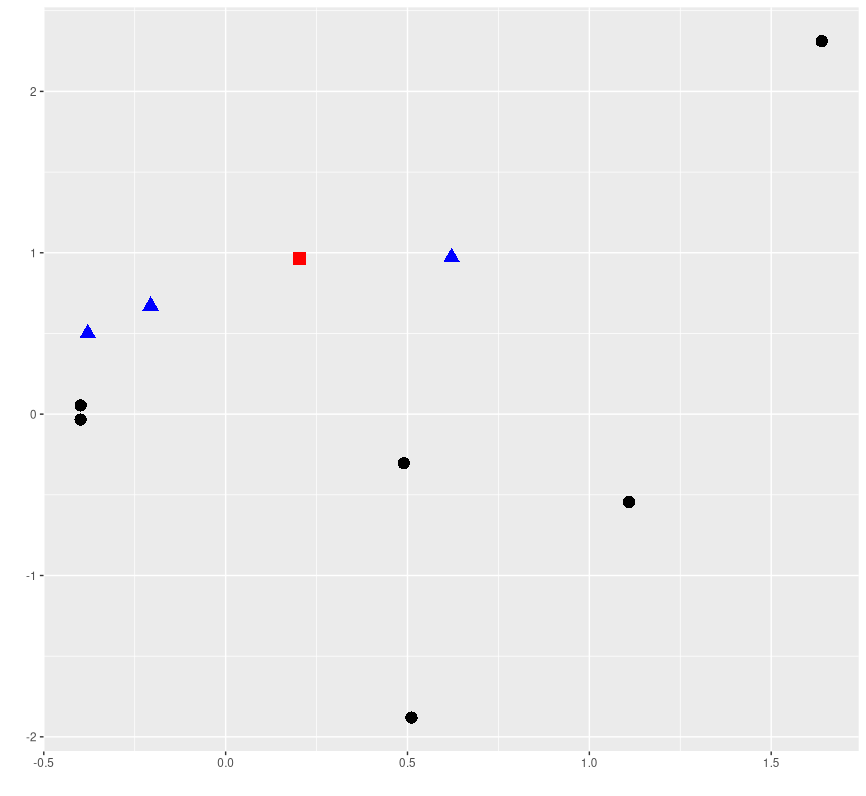
\includegraphics[scale=0.8]{figures/knn.png}
\end{center}

\end{frame}

\begin{frame}{Важность нормировки}

Расстояние \alert{чувствительно} к выбору масштаба.
\[
d(x_i, x_j) = \sqrt{(a_i - a_j)^2 + (b_i - b_j)^2 + (c_i - c_j)^2 + \ldots}  
\]

\pause

\alert{Важно} избавиться от единиц измерения!

\pause
Способ 1:
\[
a_i \to  \frac{a_i - \min(a)}{\max(a) - \min(a)}.
\]


\pause 

После преобразования все переменные лежат в отрезке $[0;1]$.

\pause

Данное масштабирование чувствительно к выбросам. 

\end{frame}


\begin{frame}{Избавиться от единиц измерения!}

  Способ 2:
  \[
  a_i \to \frac{a_i - \bar a}{\sqrt{\frac{\sum (a_i - \bar a)^2}{n - 1}}}.
  \]
  
  \pause 
  
  После преобразования каждая переменная имеет среднее равное нулю и 
  около 95\% её значений лежат в отрезке $[-2;2]$.
  
  \pause
  
  Данное масштабирование не учитывает выборочную корреляцию между переменными. 
  
\end{frame}



\begin{frame}{Избавиться от единиц измерения!}

  Способ 3: метрика Махаланобиса.
   \[
   x_i \to \left(\widehat{ \Var }(x_i)\right)^{-0.5} (x_i - \bar x)
   \]

\pause

Каждая новая переменная имеет среднее равное нулю и 
около $95\%$ её значений лежат в отрезке $[-2; 2]$.

\pause 
Новые переменные имеют нулевую выборочную корреляцию. 

\end{frame}


\begin{frame}{Как выбрать количество соседей?}

Основной способ: \alert{кросс-валидация}. 

\pause 
Для нескольких разных $k$, например, для $k \in \{1, 2, 3, 4, 5 \}$:

\begin{enumerate}[<+->]

\item Построим прогноз для каждого наблюдения, используя $k$ его ближайших соседей. 
\item Посчитаем сумму квадратов ошибок прогнозов
\[
  MSE_{k} = \frac{1}{n}\sum (y_i - \hat y_i^{cv})^2.
\]
\end{enumerate}
\pause
Выберем \alert{оптимальное} $k$.
\end{frame}



\begin{frame}{Задача классификации}


Что изменится, если $y$ — \alert{бинарная} переменная?  
\pause

Кратко: \alert{ничего}.

\pause
Зависимая переменная $y$ закодирована как $0$ и $1$, 
а $x_5$, $x_{42}$, $x_{100}$ — ближайшие наблюдения к $x$.


Считаем прогноз для вектора предикторов $x$ как среднее:
\[
\hat y = \frac{y_5 + y_{42} + y_{100}}{3}.
\]

\pause

Величина $\hat y$ — \alert{оценка вероятности} того, что $y = 1$.

\end{frame}

\begin{frame}{Метод $k$ ближайших соседей: итоги}

  \begin{itemize}[<+->]
    \item Предсказывает непрерывную или дискретную $y$.
    \item Не требует явного предположения \alert{о виде зависимости} от предикторов.
    \item Важно привести \alert{предикторы к общему масштабу}.
    \item \alert{Нет коэффициентов}, чтобы интерпретировать. 
    \item Можно комбинировать с другими методами.
  \end{itemize}
\end{frame}

